% $Id%

% ++++++++++++++++++++++++++++++++++++++++++++++++++++++++++++++++++++++++++
\newpage
\enlargethispage{1cm}
\hypertarget{appendix-menutree}{}
\section{CrypTool-Men�baum}
\label{s:appendix-menutree}

   % Eyecatcher_Neue-CrypTool-Version
Dieser Anhang enth�lt auf der folgenden Seite den kompletten Men�baum der
CrypTool\index{CrypTool}-Version 1.4.30\footnote{%
  Parallel zu CrypTool 1.x\index{CrypTool 1.x} werden im CrypTool-Projekt
  momentan auch die Zukunftsversionen CrypTool 2\index{CrypTool 2.0} und
  JCrypTool\index{JCrypTool 1.0} entwickelt.\\
  Diese Zukunftsversionen sind zur Zeit (August 2009) noch Betaversionen;
  sie sind aber schon stabil genug, um von Endbenutzern genutzt werden
  zu k�nnen. Wenn es hier Releaseversionen gibt, werden im Skript die
  entsprechenden Men�pfade und Men�b�ume erg�nzt.
}.

Welche Men�eintr�ge gerade aktiv (also nicht ausgegraut) sind, wird durch
den Typ des aktiven Dokumentenfenster bestimmt.

So ist z.~B. die Brute-Force-Analyse\index{Angriff!Brute-Force} f�r DES 
nur verf�gbar, wenn das aktive Fenster in Hexadezi"-mal-Darstellung 
ge�ffnet ist, w�hrend der Men�eintrag "`Zufallsdaten erzeugen\dots"'
immer verf�gbar ist (auch wenn kein Dokument ge�ffnet ist). 

%Folgende vier Dokumenttypen gibt es in CrypTool:
%\begin{center}
%\begin{tabular}{rl}
%\bf Codebuchstabe & \bf Dokumententyp \\
%T & Textdatei-Ansicht\\
%H & Hexadezimal-Ansicht\\
%P & Diagramm/Plot-Ansicht (Histogramm, Autokorrelation)\\
%O & OpenGL Graphics-Ansicht\\
%\end{tabular}
%\end{center}


\clearpage
\begin{figure}[hb]
\begin{center}
\vspace{-30pt}
%\frame{
%\includegraphics[scale=0.25, angle=270, viewport=200 30 2680 1420]
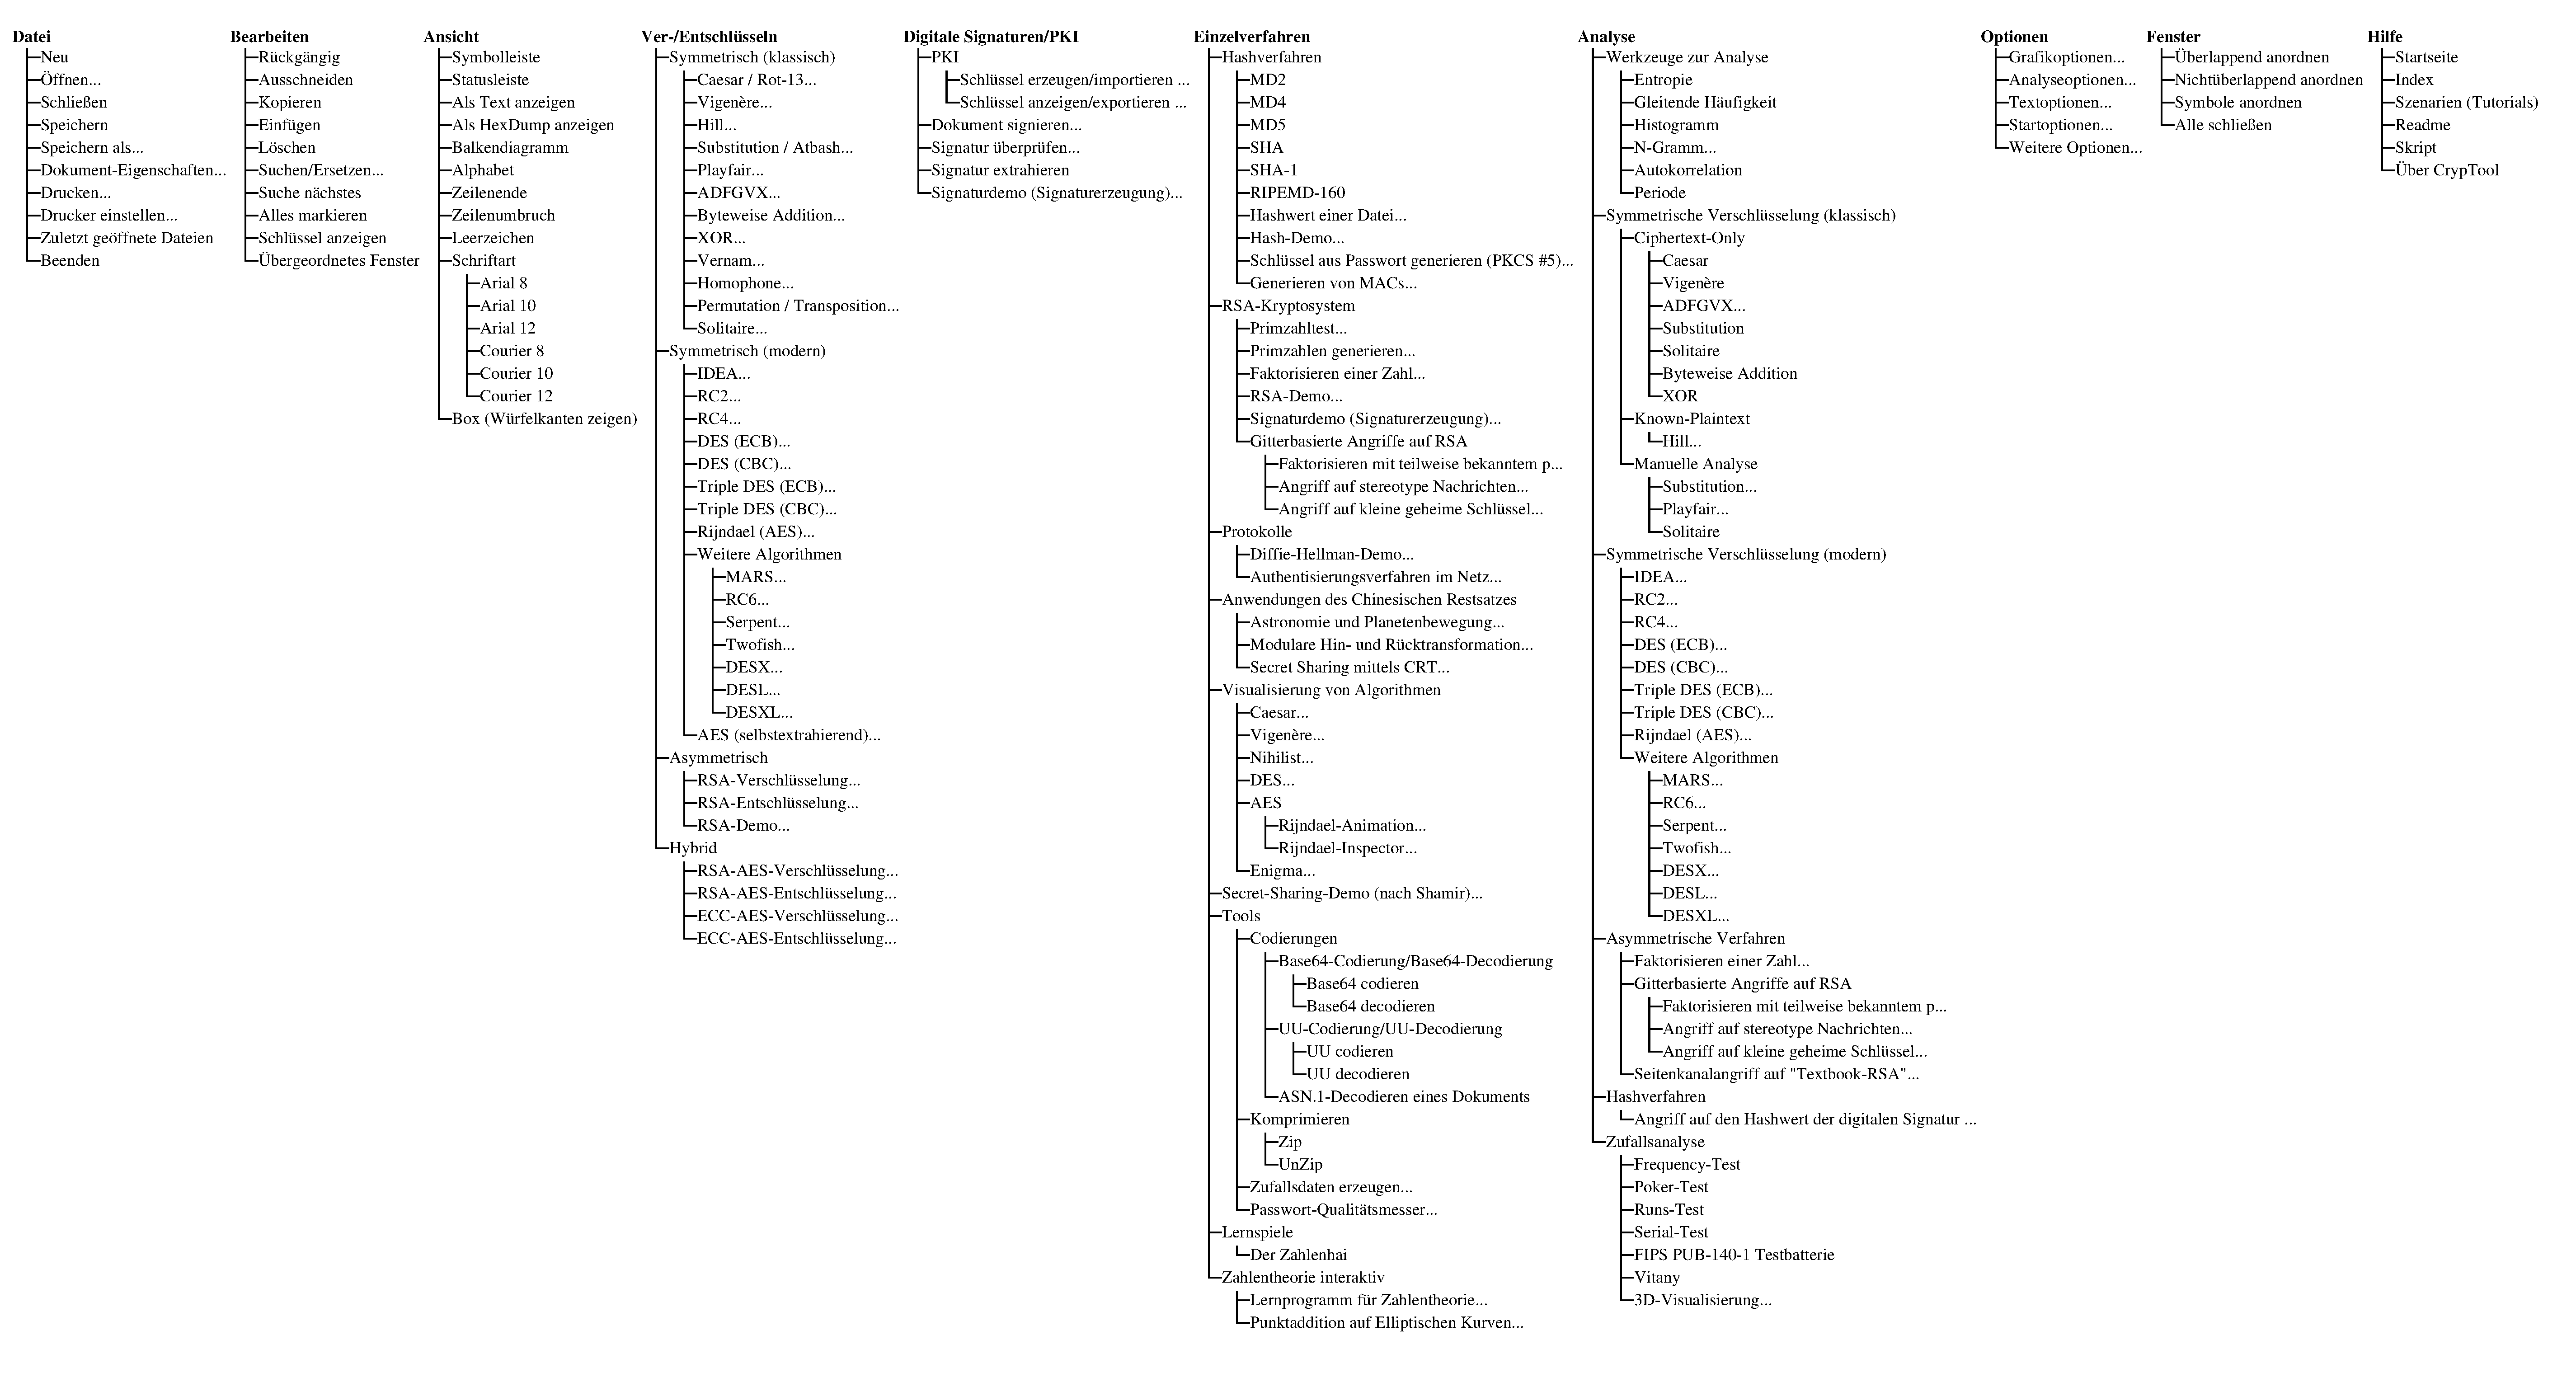
\includegraphics[scale=0.25, angle=270]
                {figures/cryptool-menu-de}
%viewport=rand-links? rand-unten breite hoehe [bezogen auf querformat]
%}
\caption{Komplette �bersicht �ber den Men�-Baum von CrypTool 1.4.30} 
\label{menuoverview}
\end{center}
\end{figure}
\clearpage

